\chapter{圆}
在工农业生产和日常生活中,圆的应用相当广泛。过去
我们初步掌握了一些圆的知识,这一章我们将在复习这些知
识的基础上,把圆和直线形结合起来,进一步学习有关圆的
一些性质。

\section{圆的基本性质}
\subsection{圆的概念}
在一个平面上和某一定点的距离等于定长的点的集合叫
做\textbf{圆周},简称为\textbf{圆};其中定点叫做圆的\textbf{圆心},连结圆心与圆
上任一点的线段叫做\textbf{半径}.通常以点$O$为圆心的圆记作$\odot O$; 
以点$O$为圆心,半径长是$r$的圆记作$\odot(O,r)$。


显然,\textbf{同圆的半径都相等}(图4.1)。而当一个圆的圆
心确定了,半径$r$的大小也确定了,这个圆的位置与大小也
就完全确定了。

圆上任意两点间的部分叫做\textbf{弧};连结圆上任意两点间的
线段叫做这个圆的弦;通过圆心的弦叫做圆的\textbf{直径}(图4.2)。
显然,\textbf{一个圆的直径等于它的半径的二倍}。
\begin{figure}[htp]\centering
    \begin{minipage}[t]{0.48\textwidth}
    \centering
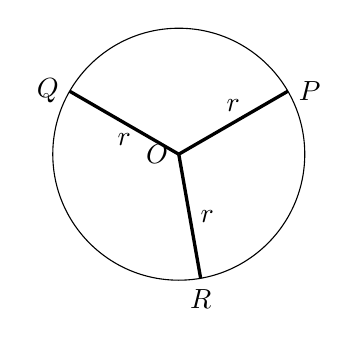
\begin{tikzpicture}[>=latex, scale=.8]
    \draw (0,0) circle (2);
\draw[very thick](0,0)node[left]{$O$}--node[above]{$r$}(30:2)node[right]{$P$};
\draw[very thick](0,0)--node[below]{$r$}(150:2)node[left]{$Q$};
\draw[very thick](0,0)--node[right]{$r$}(-80:2)node[below]{$R$};
    \end{tikzpicture}
    \caption{}
    \end{minipage}
    \begin{minipage}[t]{0.48\textwidth}
    \centering
    \begin{tikzpicture}[>=latex, scale=.8]
        \draw  (0,0) circle (2);
\draw[very thick] (60:2)--node[below]{弦}(135:2);
\draw[very thick] (-10:2)--node[below]{直径}(170:2);
\draw (-135:2) [fill=black]circle(1.5pt)node[left]{$E$};
\draw (-45:2) [fill=black]circle(1.5pt)node[right]{$F$};
\draw[very thick]  (-135:2) arc (-135:-45:2);
\node at (0,-2) [below=2pt]{弧};


    \end{tikzpicture}
    \caption{}
    \end{minipage}
    \end{figure}

从圆的定义,不难直接推知:
\begin{itemize}
    \item 两个圆能够重合的充要条件是两个圆的半径相等。
    \item 半径相等的圆叫做\textbf{等圆},\textbf{等圆的半径相等直径相等}。
\end{itemize}

从圆的定义,我们还可以看出,一个圆把它所在的平面
分为三部分(图4.3):
\begin{enumerate}
    \item 圆本身,即与圆心的距离等于半径的点所构成的集
合。其中任何一点都叫做圆上的点。
\item 圆的内部,与圆心的距离小于半径的点所构成的集
合。圆的内部又简称\textbf{圆内};其中任何一点都叫做圆内的点。
\item 圆的外部:与圆心的距离大于半径的点所构成的集
合;圆的外部又简称\textbf{圆外},其中任何一点都叫做圆外的点。
\end{enumerate}

\begin{figure}[htp]\centering
    \begin{minipage}[t]{0.48\textwidth}
    \centering
\begin{tikzpicture}[>=latex, scale=.8]
    \draw[pattern=north west lines] (0,0) circle (2);
    \draw[thick] (0,0)--node[left=3.5pt, fill=white]{$r$}(60:2);
    \end{tikzpicture}
    \caption{}
    \end{minipage}
    \begin{minipage}[t]{0.48\textwidth}
    \centering
    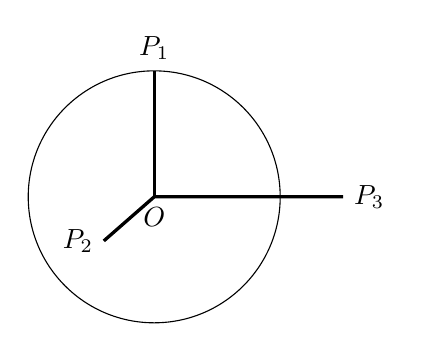
\begin{tikzpicture}[>=latex, scale=.8]
        \draw  (0,0) circle (2);
\draw[very thick](-.8,-.7)node[left]{$P_2$}--(0,0)node[below]{$O$}--(3,0)node[right]{$P_3$};
\draw[very thick](0,0)--(0,2)node[above]{$P_1$};

    \end{tikzpicture}
    \caption{}
    \end{minipage}
    \end{figure}

通常我们说的圆面,指的是由圆所围成的平面部分,也
就是与圆心的距离小于或等于半径的点所构成的集合。如图
4.3中阴影部分。

由上述定义可知,$\odot(O,r)$与平面上任一点P的位置关
系,有下述的性质(图4.4)。
\begin{enumerate}
    \item 点$P$在$\odot(O,r)$上的充要条件是$\overline{OP}=r$;
    \item 点$P$在$\odot(O,r)$内的充要条件是$\overline{OP}<r$;
    \item 点$P$在$\odot(O,r)$外的充要条件是$\overline{OP}>r$。
\end{enumerate}

\begin{ex}
\begin{enumerate}
    \item 根据下述条件画圆
\begin{enumerate}
\item 已知定点$O$, 以$O$为圆心画一圆使半径等于2厘
米。
\item 已知两个定点$O$、$P$, 画$\odot(O,\overline{OP})$.
\item 先画一条$\overline{AB}$, 再画出以$\overline{AB}$
为直径的圆。
\end{enumerate}

\item 把以下命题写成“若一则”形式
\begin{enumerate}
\item 点$P$在$\odot(O,r)$上的充分条件是
$\overline{OP}=r$;
\item 点$P$在$\odot(O,r)$内的必要条件是
$\overline{OP}<r$;
\item 点$P$在$\odot(O,r)$外的充分条件是
$\overline{OP}>r$。
\end{enumerate}


\item 以点$O$为圆心,$r_1$、$r_2$为半径画两个圆。说出满足下列条
件的点$X$在平面上的位置范围。
\begin{multicols}{2}
\begin{enumerate}
    \item $\overline{OX} >r_2$
    \item $\overline{OX} \le r_1$
    \item $r_1<\overline{OX}<r_2 $
    \item $\overline{OX}=r_1 $
    \item $\overline{OX}<r_1 $
\end{enumerate}
\end{multicols}

\item 已知一个$\odot O$的直径长是4cm. 说出满足下列条件的$P$点
的可能位置:
\begin{multicols}{2}
    \begin{enumerate}
        \item $\overline{OP} >2$cm
        \item $\overline{OP} \ge 2$cm
        \item $\overline{OP} <2$cm
        \item $\overline{OP} =0$
    \end{enumerate}
    \end{multicols}

\item 求证一个圆的直径
是这个圆中最长的弦。

(提示:按图中所示证$\overline{AB}>\overline{CD}$)。
\begin{center}
    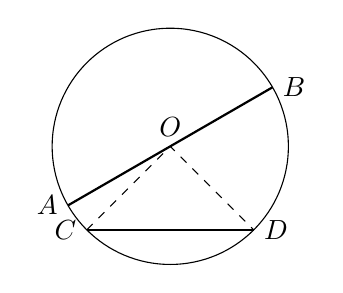
\begin{tikzpicture}
        \draw (0,0) circle (1.5);
\draw[thick] (-150:1.5)node[left]{$A$}--node[above]{$O$}(30:1.5)node[right]{$B$};
\draw[thick]  (-135:1.5)node[left]{$C$}--(-45:1.5)node[right]{$D$};
\draw[dashed](-135:1.5)--(0,0)--(-45:1.5);
    \end{tikzpicture}
\end{center}
\end{enumerate}
\end{ex}

\subsection{不共线的三点确定一圆}
我们已知,如果知道了圆心的位置和半径长,那么圆的
位置和大小也就确定了。现在我们来研究经过一个点;经过
两个点;经过三个点可分别作出几个圆?
    
已知一个点$A$, 很明显,以$A$点以外的任何点为圆心,
以这点到$A$点的距离为半径所作的圆都经过$A$点(图4.5)。
因此,\textbf{经过一点可以作无数个圆}。

经过两个已知点$A$、$B$,可以作多少个圆呢(图4.6)?
由于经过$A$、$B$两点的圆的圆心到$A$点与$B$点的距离应相等,而
和$A$、$B$两点距离相等的点仅在$AB$的垂直平分线上,所以,
以$AB$的垂直平分线上任一点为圆心,以这点到$A$点(或$B$
点)的距离为半径所作的圆都经过$A$、$B$两点。因此,\textbf{经过
两点也可以作无数个圆,且圆心都在连结这两点的线段的垂
直平分线上}。

现在我们来研究,经过$A$、$B$、$C$三点可以作多少个圆的
问题?




























